\section{Interpretation}
\label{sec:interpretation}

In this section, we interpret the results of the targeted search in the context of the \wzmet\ model depicted in Fig.~\ref{fig:diagrams} (right)
and a gauge-mediated SUSY breaking (GMSB) model that produces a signature of \zzmet\ will be added. The results of the targeted search presented here
will be combined with those of the trilepton ewkino search for the final \wzmet\ interpretation, and with the quadlepton ewkino search
for the final GMSB \zzmet\ interpretation.

The exclusion is performed using the results of simultaneous counting experiments in the five exclusive \MET\ signal regions defined by \MET\ $>$ 80 GeV,
as summarized in Table~\ref{tab:results_targ} (commonly referred to as a ``shape analysis''). 
The upper limit calculation is performed with the LandS software using the LHC-type CLs criterion.
The signal efficiency uncertainties include the luminosity (4.4\%), acceptance for the b-jet veto (4\%), lepton ID and isolation efficiency (2\% per lepton),
and trigger efficiency (3\%). The uncertainty from JES is determined following the POG-recommended procedure, by varying the jet energies by the 
\pt- and $\eta$-dependent uncertainties and propagating this to the jet multiplicity, dijet mass, and \MET.
The background uncertainties are quoted in Table~\ref{tab:results_targ}. For each background contribution, the uncertainty is assumed to be 100\% 
correlated across all signal regions.

For the \wzmet\ model, the signal efficiency times acceptance and cross section upper limits are displayed in Fig.~\ref{fig:results_wzmet},
along with the observed and expected exclusion contours, which are compared to the 2011 observed exclusion contour.
Figure~\ref{fig:results_wzmetpoints} shows the excluded points used to derive the exclusion contours. We note that the map of exclusion
contours appears quite ragged since for many of the points the cross section upper limit is very close to the theory cross section.
Therefore we do not expect the ragged exclusion region to be an issue for the final results since
we currently have 9.2 fb$^{-1}$ and expect the luminosity to increase significantly. A {\bf VERY APPROXIMATE} projection of the expected excluded region
for an integrated luminosity of 15 fb$^{-1}$ (a rough guess at the final HCP data sample) is obtained by scaling the expected cross section limits by 
$\sqrt{(9.2 \rm{fb}^{-1})/(15 \rm{fb}^{-1})}$, as displayed in Fig.~\ref{fig:results_15fb}.

\begin{figure}[!ht]
\begin{center}
\begin{tabular}{cc}
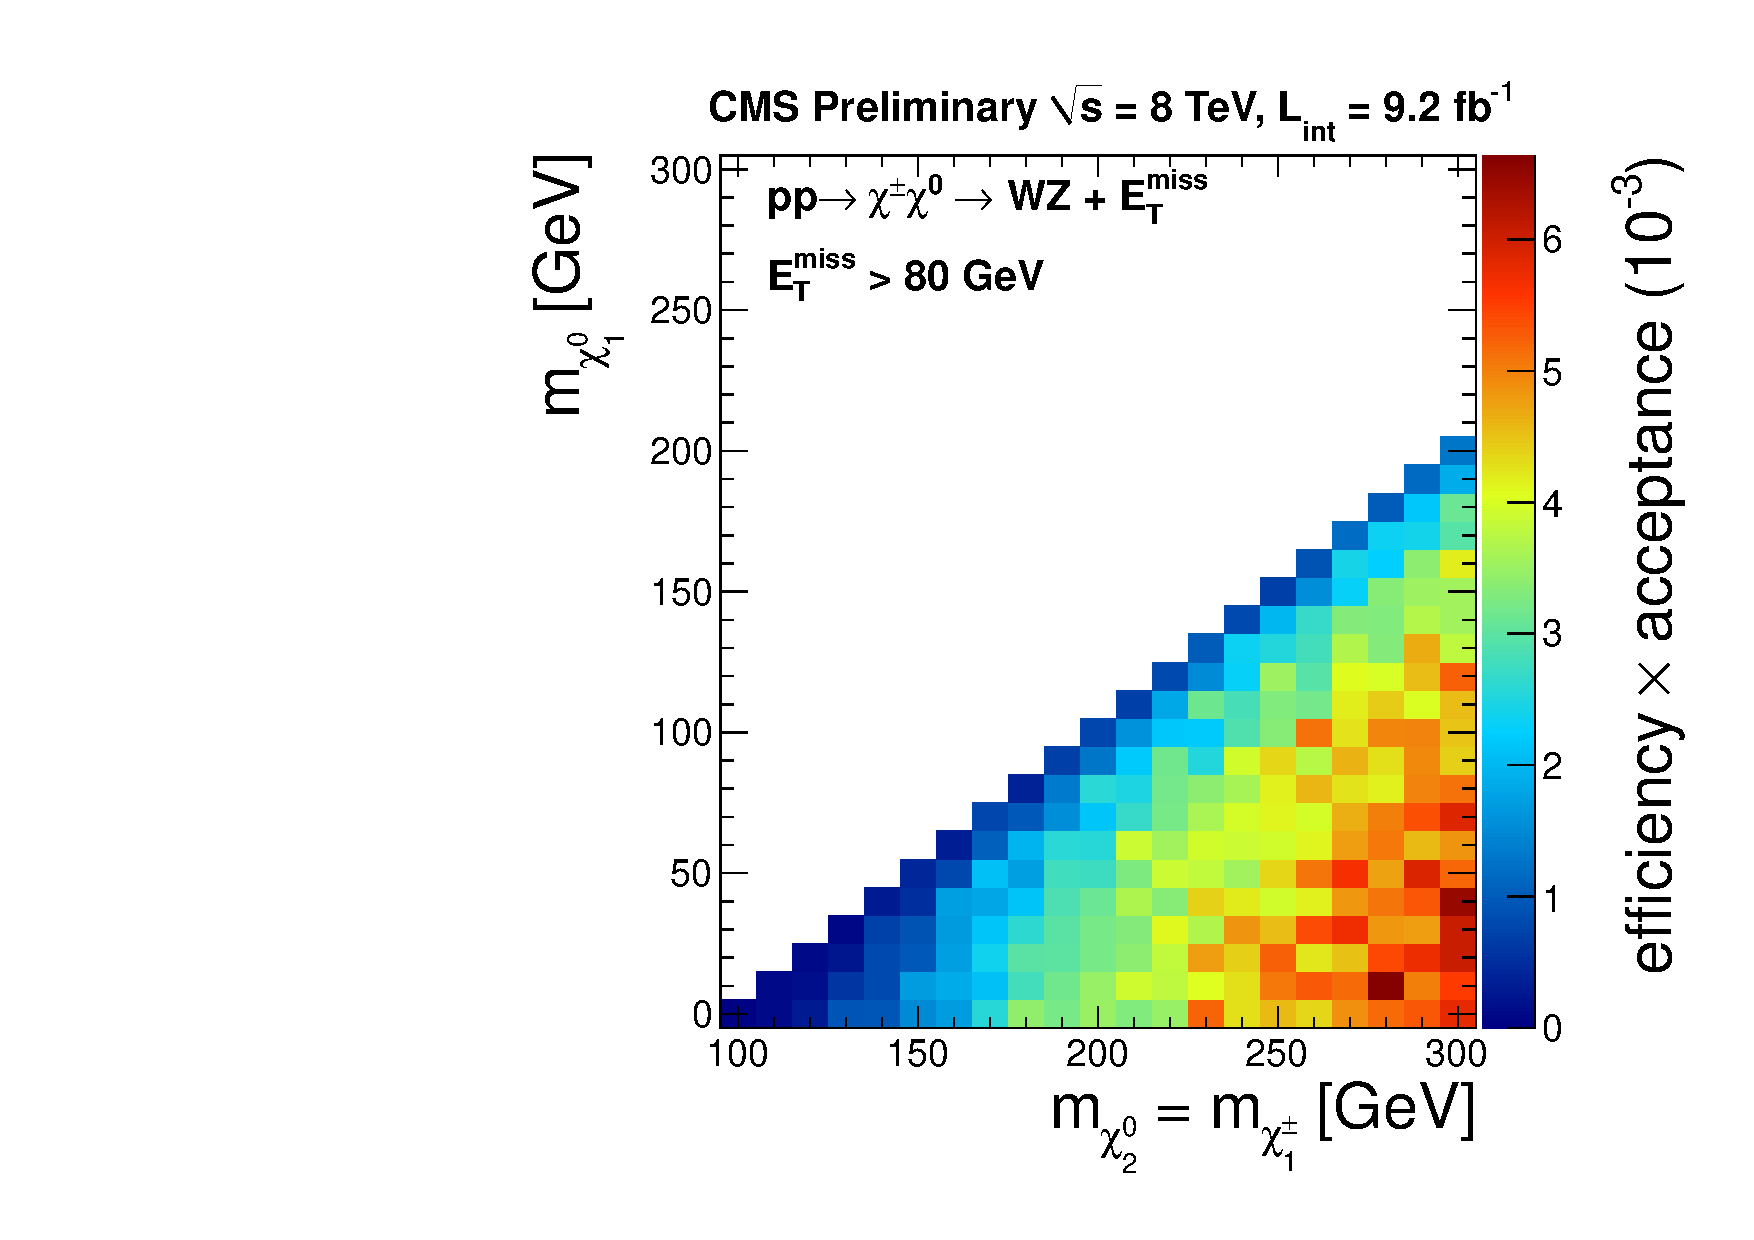
\includegraphics[width=0.45\textwidth]{plots/wzsms_eff.pdf}
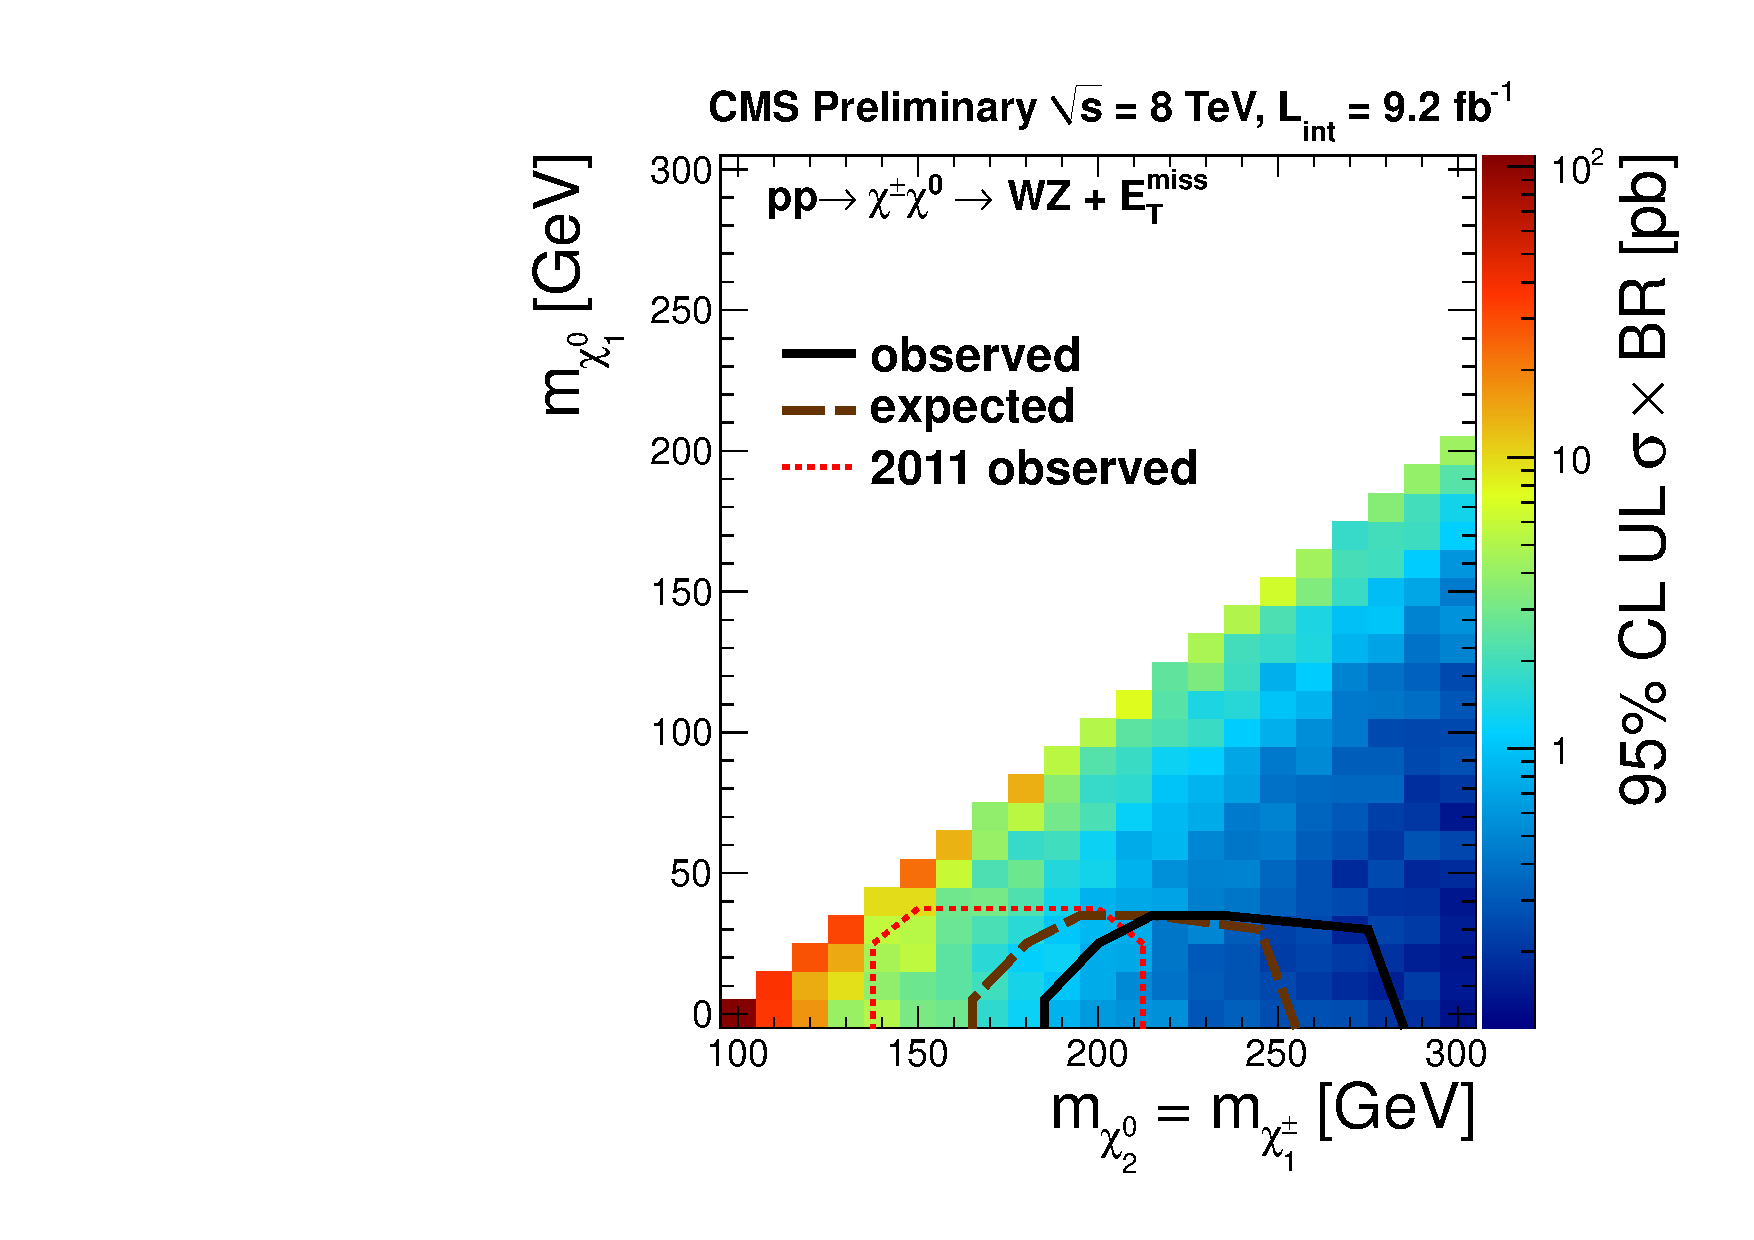
\includegraphics[width=0.45\textwidth]{plots/wzsms_xsec.pdf}
\end{tabular}
\caption{ Interpretation of the targeted analysis in the \wzmet\ model. The acceptance times efficiency (left) and cross section
upper limit (right) and displayed. The observed and expected exclusion contours are indicated and compared to the observed
exclusion from the 2011 analysis.
\label{fig:results_wzmet}}
\end{center}
\end{figure}

\begin{figure}[!hb]
\begin{center}
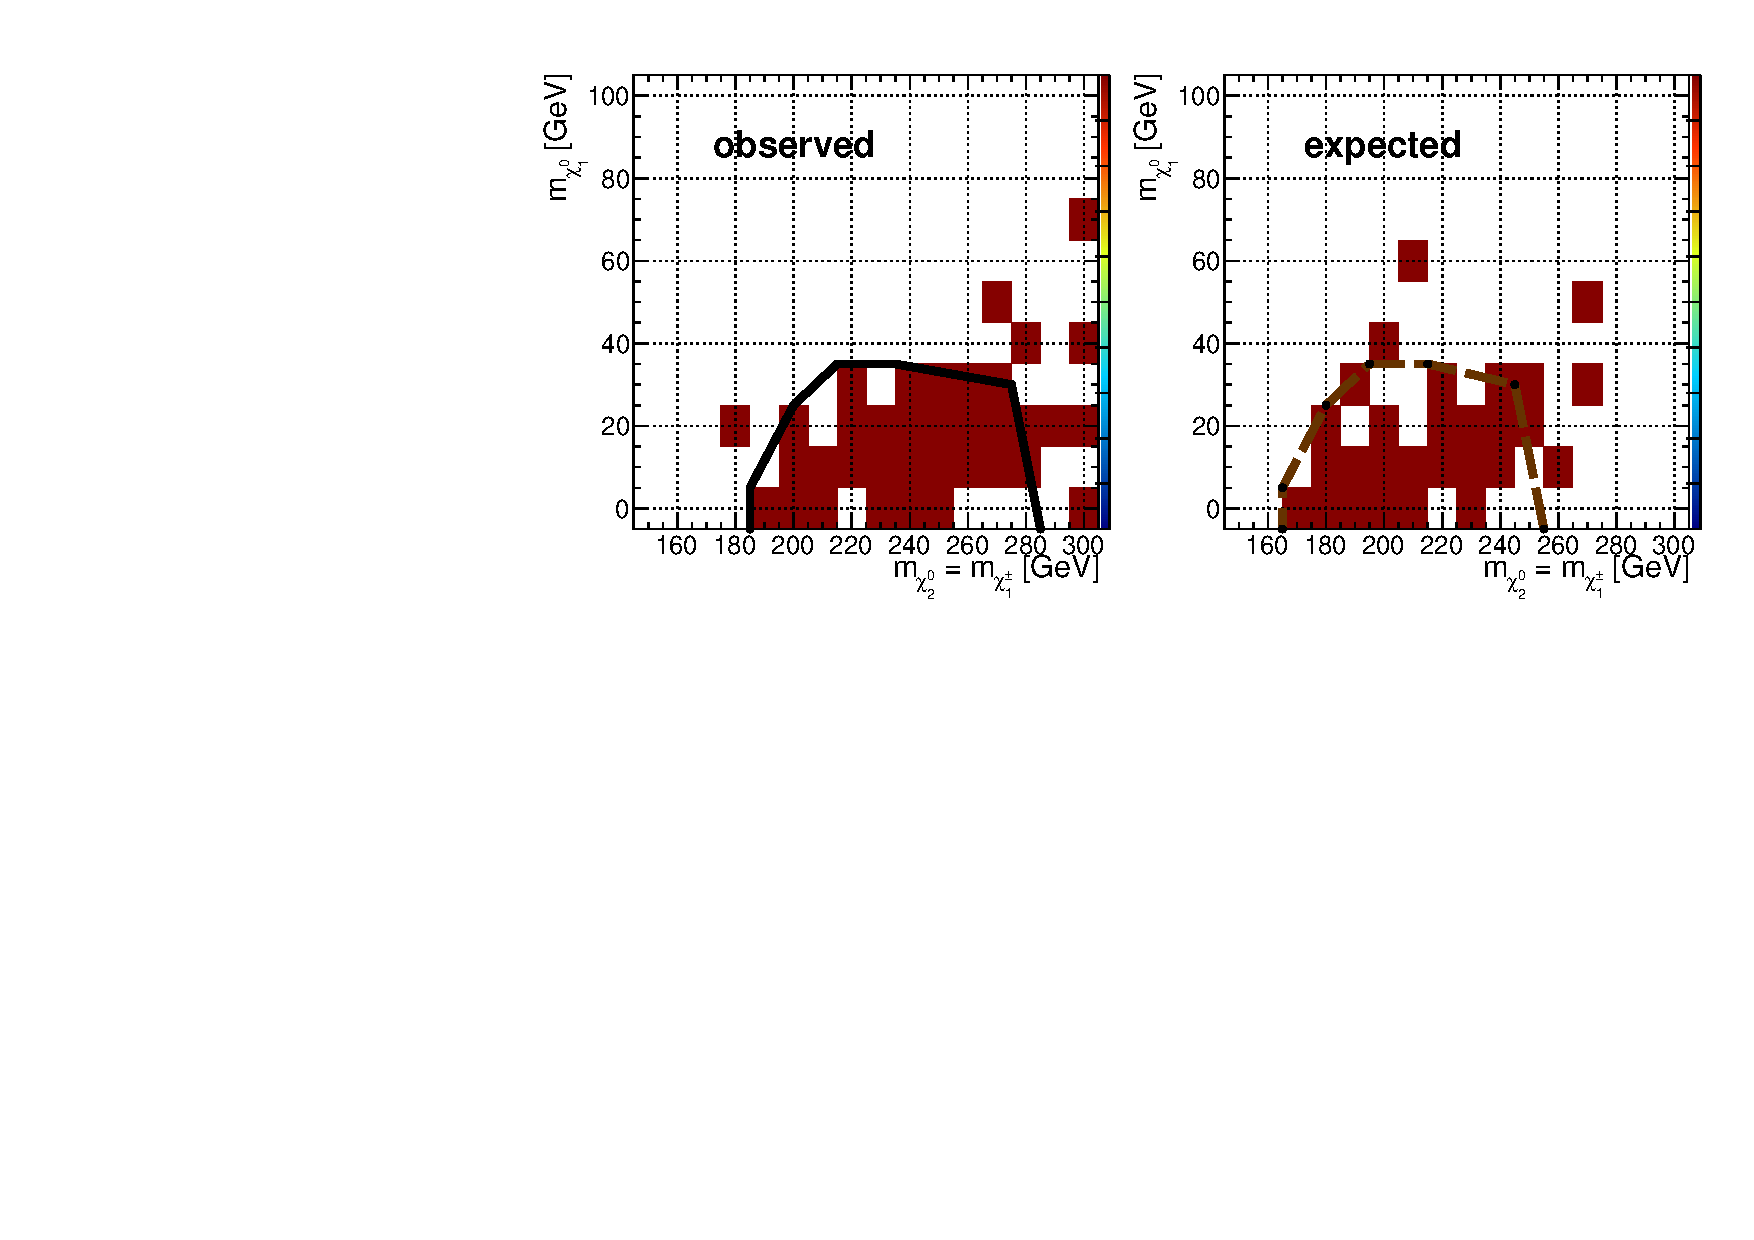
\includegraphics[width=0.75\textwidth]{plots/wzsms_points.pdf}
\caption{ Observed (left) and expected (right) excluded points for the \wzmet\ interpretation, with the corresponding exclusion contours overlaid.
\label{fig:results_wzmetpoints}}
\end{center}
\end{figure}

\clearpage

\begin{figure}[!ht]
\begin{center}
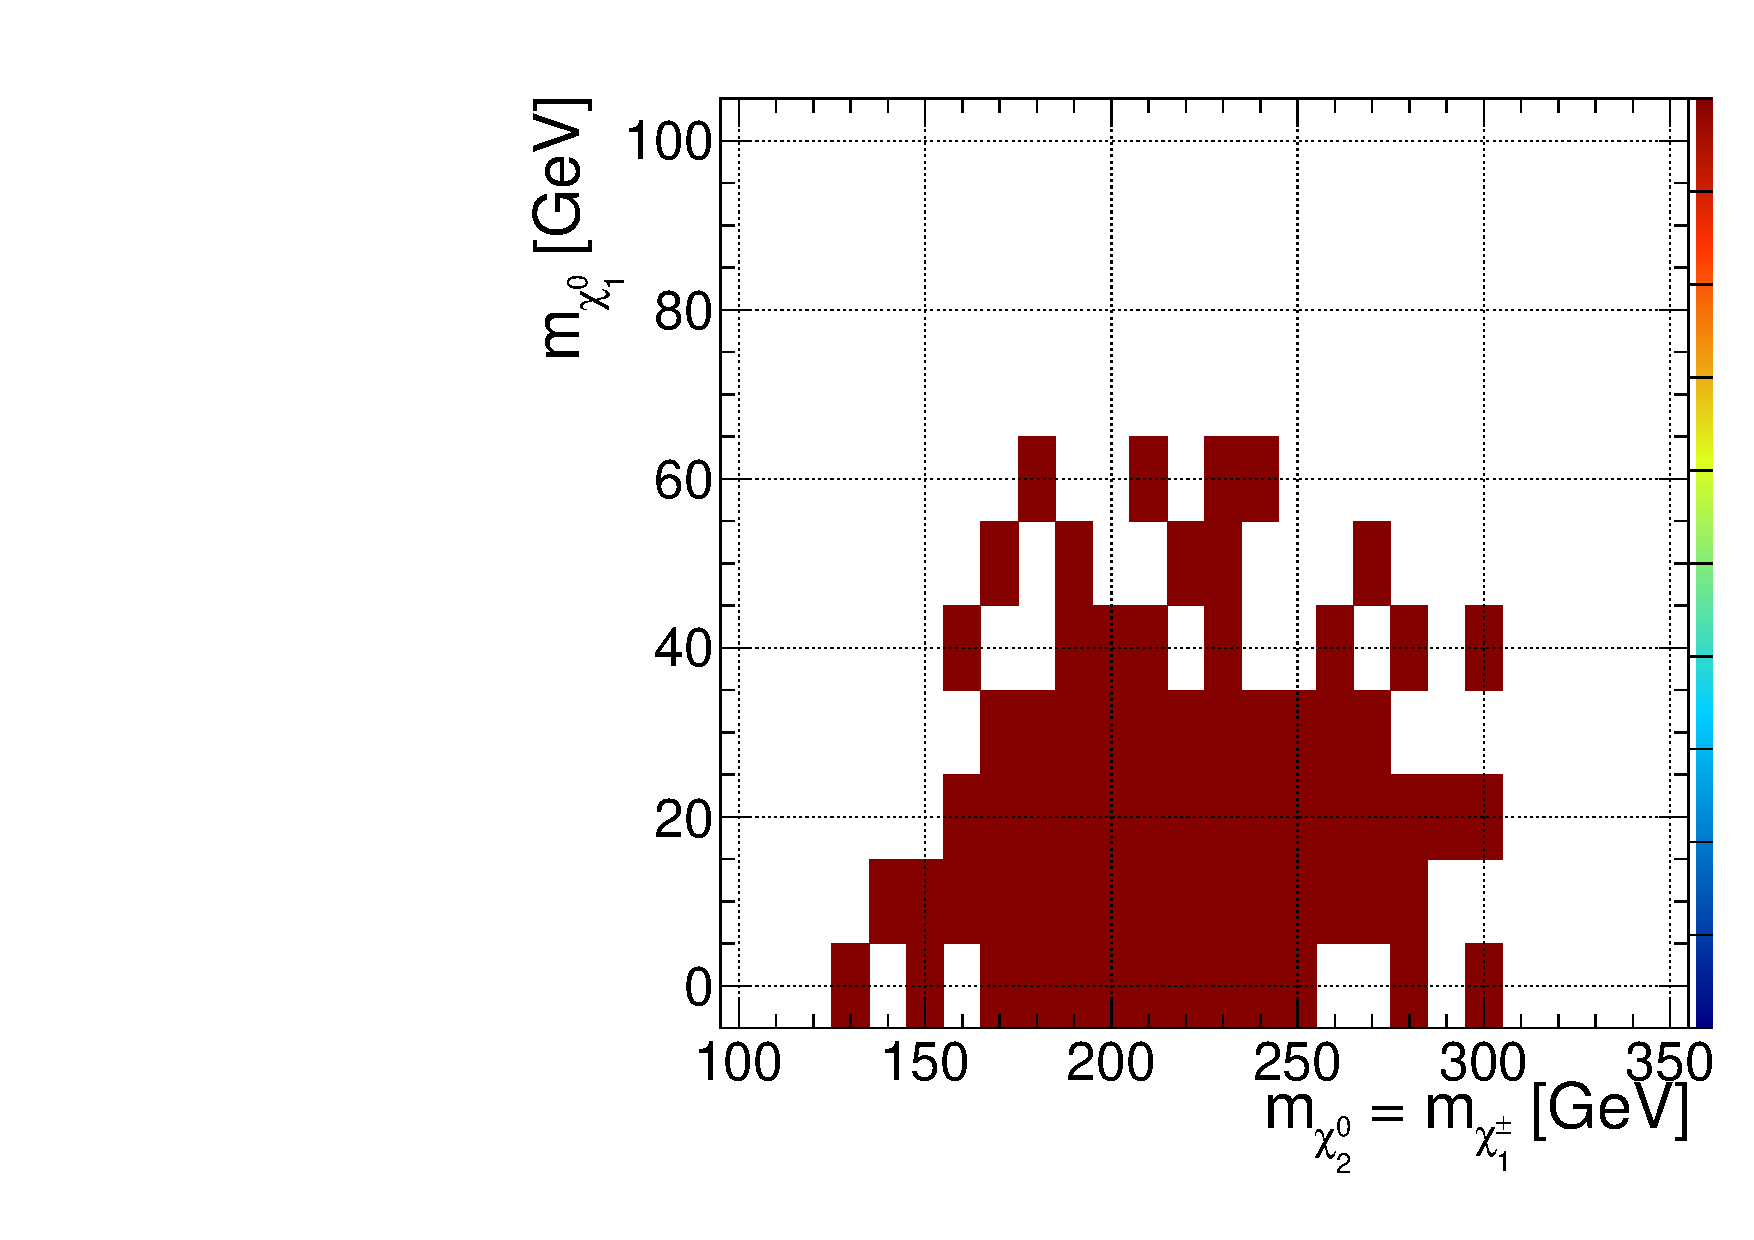
\includegraphics[width=0.5\textwidth]{plots/wzsms_expected_15fb.pdf}
\caption{ A {\bf VERY APPROXIMATE} projection of the expected excluded points for an integrated luminosity of 15$^{-1}$. 
\label{fig:results_15fb}}
\end{center}
\end{figure}

The results of the interpretation in the GMSB \zzmet\ model are displayed in Fig.~\ref{fig:results_gmsb},
as a function of the chargino and neutralino mass parameter $\mu$. These results exclude the range $196 < \mu < 316$~GeV.

\begin{figure}[!hb]
\begin{center}
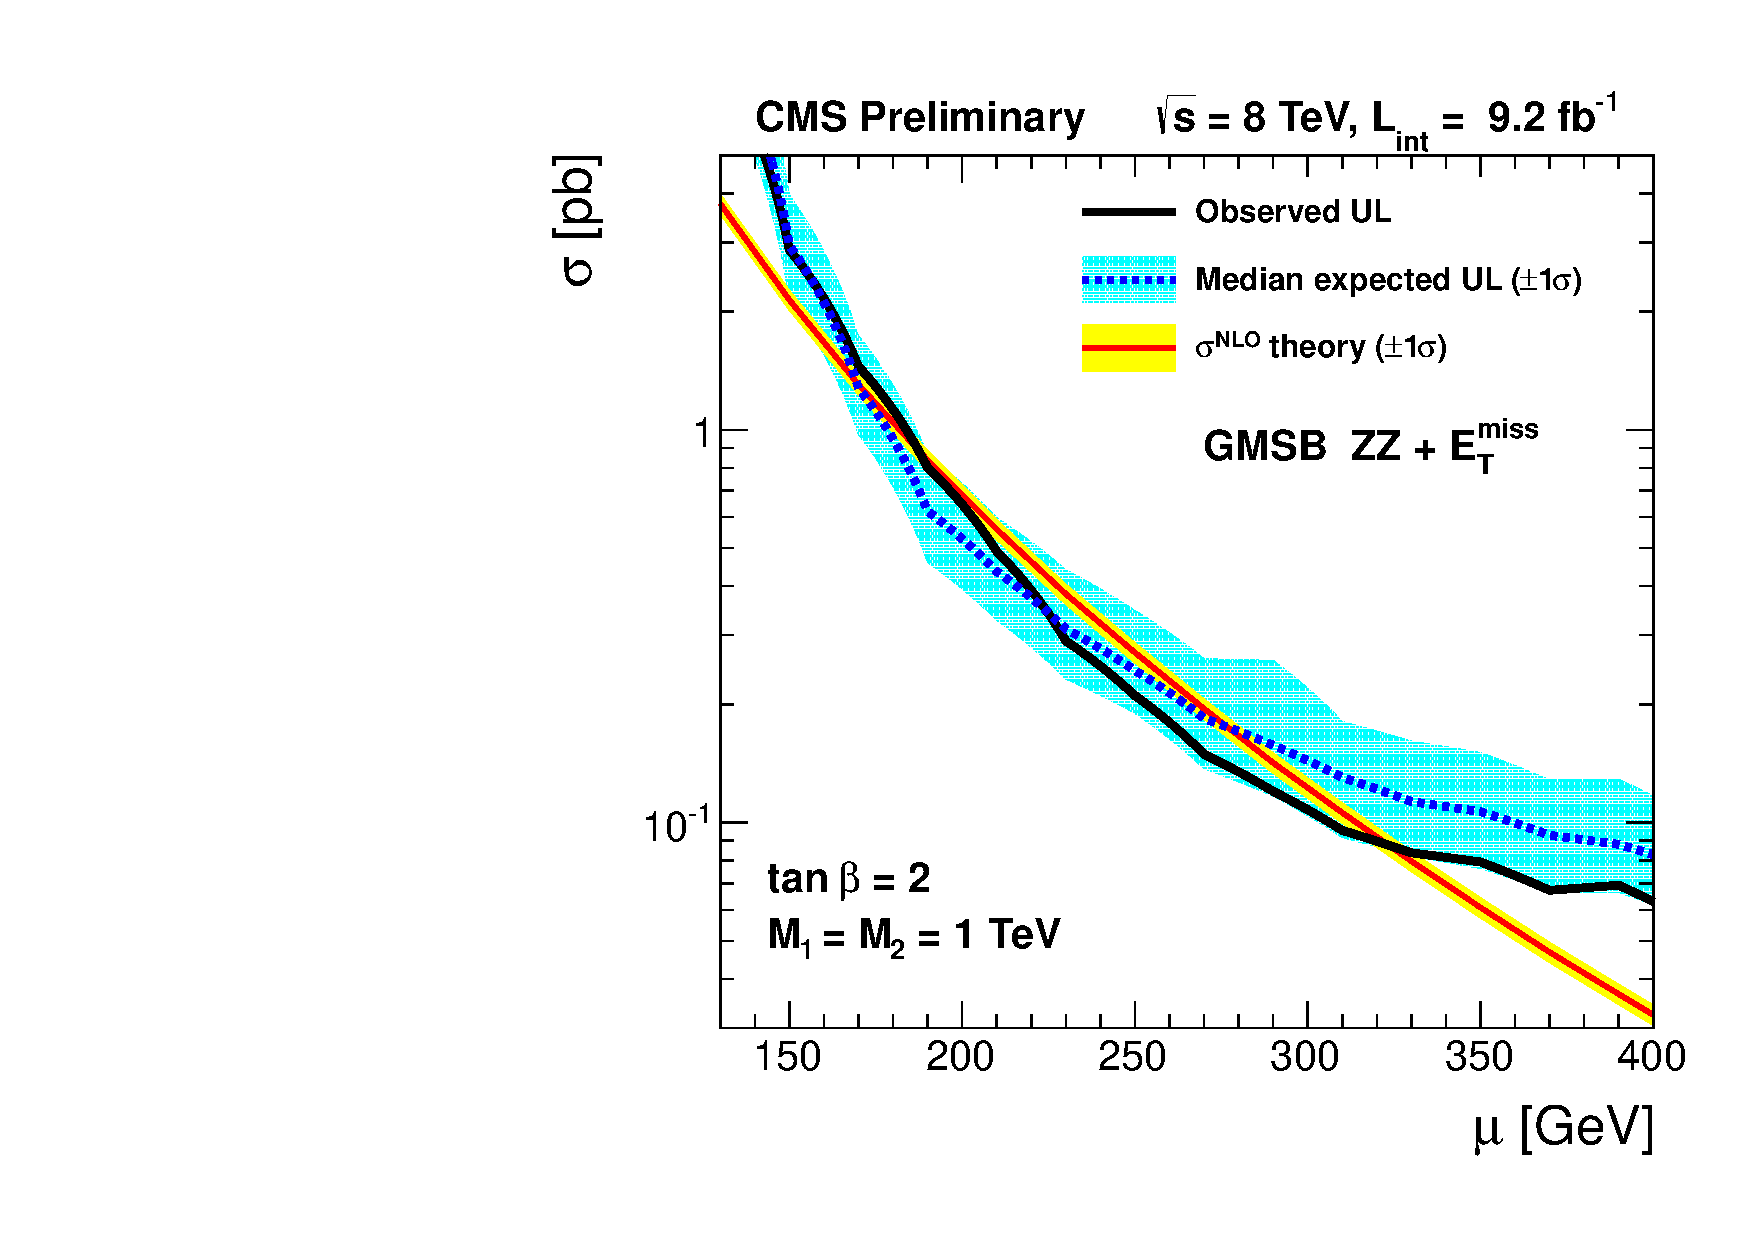
\includegraphics[width=0.5\textwidth]{plots/ZDIJET_GMSB.pdf}
\caption{ Interpretation of the targeted analysis in the GMSB \zzmet\ model.
\label{fig:results_gmsb}}
\end{center}
\end{figure}
